\documentclass{article}

\usepackage[final]{nips2016}
\usepackage{subcaption}
\usepackage{epstopdf}
\usepackage{graphicx}
\usepackage[utf8]{inputenc}
\usepackage[T1]{fontenc}
\usepackage{hyperref}
\usepackage{url}
\usepackage{booktabs}
\usepackage{amsfonts}
\usepackage{nicefrac}
\usepackage{microtype}
\usepackage{amsmath}
\usepackage{amssymb}
\usepackage{algorithm}
\usepackage[noend]{algpseudocode}
\graphicspath{{images/}}

\newcommand{\specialcell}[2][c]{%
  \begin{tabular}[#1]{@{}c@{}}#2\end{tabular}}

\title{Human Activity Recognition with HMMs}

% The \author macro works with any number of authors. There are two
% commands used to separate the names and addresses of multiple
% authors: \And and \AND.
%
% Using \And between authors leaves it to LaTeX to determine where to
% break the lines. Using \AND forces a line break at that point. So,
% if LaTeX puts 3 of 4 authors names on the first line, and the last
% on the second line, try using \AND instead of \And before the third
% author name.

\author{
  William Jow \\
  2nd year undergraduate \\
  \texttt{williamjow@berkeley.edu}
  \and
  \textbf{David Lin} \\
  3rd year undergraduate \\
  \texttt{lin.david@berkeley.edu}
  \and
  \textbf{Owen Jow} \\
  4th year undergraduate \\
  \texttt{owenjow@berkeley.edu}
}

\begin{document}
\maketitle

\begin{abstract}

In this project, we explore applications of hidden Markov models (HMMs) in the context of human activity recognition. We frame the recognition problem as a multinomial classification instance, where our model is given a video as input and must associate it with one of a predetermined set of activities. In building a model, we first extract per-sequence feature matrices from a training corpus of videos and subsequently run the EM algorithm on per-class HMMs in order to fit their parameters to each class's features. Later, we extend MLE-based evaluation using normalization and ensemble methods. Our algorithm produces models with 50-80\% classification accuracy on a test set, vastly outperforming the baseline 17\% given by uniform random sampling.

\end{abstract}

\section{Introduction}

Activity recognition is an active area of research in computer vision, and has applications in a wide range of domains (including healthcare, HCI, and real-time surveillance carried out by oppressive totalitarian regimes). In the modern era, typical cutting-edge methods (e.g. \cite{cz2017}, \cite{bwmt2018}, \cite{lyc2017}) ride the deep learning wave and develop fancy statistical ML formulations that involve buzzwords such as ``convolutional neural networks" and "LSTMs." In this report, however, we take a step backward and argue that \textit{Markov chains are all you need}~\footnote{to attain 50\% accuracy}, training a hidden Markov model (HMM)-based classifier on a dataset of a few hundred videos in order to achieve surprisingly decent results.

More specifically, we consider (human) activity recognition as a multinomial classification problem and build a model based on multiple HMMs, one for each activity, where the job of the aggregate model is to take a video of a human doing something and decide whether the human is (a) walking, (b) running, or so on. Each HMM is trained to represent the sequential progression of a single activity.

To engineer each HMM, we first extract centroid, edge, and optical flow features from all training videos corresponding to that HMM's activity, and then run the expectation-maximization (EM) algorithm to determine the MLE of the HMM's parameters given the set of observed feature vectors. After training each HMM in this fashion, we can evaluate the overall model on a video by having each HMM score the video's feature representation and then choosing the activity whose HMM produces the highest score. We also find slight improvement through normalization and ensemble methods, in which we (a) attempt to enforce that the output distributions of each HMM resemble each other in first and second central moments and (b) train multiple HMMs for each activity and average their outputs.

We evaluate our algorithm on the KTH action dataset \cite{slc2004}, which contains several hundred videos of six activity classes over homogeneous backgrounds. In contrast to uniform random sampling, which gives an expected 17\% classification accuracy, our method classifies each activity with 50-80\% accuracy on a separate test set. Meanwhile, despite some variability in performance, ensemble models are shown to slightly outperform vanilla models in classifying most activities.

\section{Background}

\subsection{HMMs}\label{sec:hmms}

Our method uses a hidden Markov model in order to predict the correct activity. The hidden Markov model or HMM is a sequence classifier that assigns a label to each item in a sequence. The hidden Markov model uses an underlying Markov chain, which is a sequence of variables in which the probability of an event is dependent only on the prior state. Given a sequence of observations, the HMM computes a probability distribution over the possible label sequences and selects the best one. 

An HMM relies on three components: a transition probability distribution, an observation likelihood distribution, and an initial state distribution. The transition distribution describes the distribution for the next state given the current state. The observation distribution describes the distribution of the output given the current state. Finally, the initial state distribution describes the starting distribution over the states. Together, these properties allow the HMM to compute the probability for any sequence of events.

An HMM also has two core algorithms to help determine the likelihood of an observation given an HMM and learn the HMM parameters.

\subsection{The Forward Algorithm}\label{sec:forward-alg}

The forward algorithm is used to compute the likelihood of a certain observation sequence. The algorithm uses dynamic programming to compute the observation probability by summing over the probabilities of all possible hidden state paths that could generate the observation sequence. To compute the forward probability, the previous forward path probability, the transition probability, and the state observation likelihood are multiplied together in each step. The pseudocode of this algorithm is as follows:

\begin{quote}
Where $\alpha_t(j) = \text{forward}[j, t]$ denotes the probability of being in state $j$ after observing the first $t$ observations, $a_{i,j}$ denotes the transition probability from state $i$ to state $j$, $b_j(o_t)$ denotes the probability of observing $o_t$ given the current state is $j$, and $s_F$ is the final state,
\begin{algorithm}
\caption{Forward Algorithm}
\begin{algorithmic}
    \Procedure{Forward}{observations length $T$, state graph length $N$}
    \State initialize forward[$N$, $T$]
    \For{each state $s$ from 1 to $N$}
        \State forward[$s$, 1] $\gets$ $a_{0, s} \cdot b_s (o_1)$
    \EndFor
    \For{each time step $t$ from 2 to $T$}
        \For{each state $s$ from 1 to $N$}
            \State forward[$s$, $t$] $\gets$ 
            $\displaystyle \sum_{s' = 1}^{N} \text{forward}[s', t - 1]
                                             \cdot a_{s', s} \cdot b_s(o_t)$
        \EndFor
    \EndFor
    \Return $\sum_{s = 1}^{N} \text{forward}[s, T] \cdot a_{s, s_F}$
    \EndProcedure
\end{algorithmic}
\end{algorithm}

In our implementation, we take the log of each probability and thus perform addition where there is multiplication above.
\end{quote}

% \subsection{The Viterbi Algorithm}\label{sec:viterbi-alg}

% The Viterbi algorithm is used to determine which sequence of variables is the hidden source of the sequence of observations. The algorithm uses dynamic programming to calculate the hidden state sequence with the maximum observation likelihood from the forward algorithm.

\subsection{The Forward-Backward Algorithm}\label{sec:bw-alg}

The forward-backward or Baum-Welch algorithm, a special case of the Expectation-Maximization (EM) algorithm, is used to learn the parameters of an HMM. The algorithm allows us to train the transition and emission probabilities of the HMM. It iteratively improves on the probability estimates that it learns. Given a sequence of observations and emissions, the algorithm computes the posterior marginals of all hidden state variables. It relies on calculating the forward and backward probabilities in order to compute the transition probability and observation probability. The pseudocode of this algorithm is as follows:

\begin{quote}
Where $\xi_t(i, j)$ denotes the probability of being in state $i$ at time $t$ and state $j$ at time $t + 1$, $\gamma_t(j)$ denotes the probability of being in state $j$ at time $t$, and backward probability $\beta_t(i)$ denotes the probability of observing the observations from time $t + 1$ onward given the current state is $i$,
\begin{algorithm}
\caption{Forward-Backward Algorithm}
\begin{algorithmic}
    \Procedure{Forward-Backward}{observations length $T$, observation set $V$}
    \State initialize transition matrix $A$, observation distribution $B$
    \Repeat
        \ForAll{$t, j$}
            $\displaystyle \gamma_t(j) = \frac{\alpha_t(j) \beta_t(j)} {\alpha_T(s_F)}$
        \EndFor
        \ForAll{$t, i, j$}
            $\displaystyle \xi_t(i, j) = \frac{\alpha_t(i) a_{ij} b_j(o_{t + 1}) \beta_{t + 1}(j)} {\alpha_T(s_F)}$
        \EndFor
        
        \State $A_{ij}$ $\gets$ 
        $\displaystyle \quad \left(\sum\limits_{t = 1}^{T - 1} \xi_t(i, j)\right)/
                            \left(\sum\limits_{t = 1}^{T - 1} \sum\limits_{k = 1}^{N} \xi_t(i, k)\right)$
        \\
        \State $B_{j}(v_k)$ $\gets$
        $\displaystyle \quad \left(\sum\limits_{\substack{t = 1 \\ \text{s.t. } o_T = v_k}}^{T} \gamma_t(j)\right) / \left(\sum\limits_{t = 1}^{T} \gamma_t(j)\right)$
        \\
    \Until{convergence}
    \EndProcedure
\end{algorithmic}
\end{algorithm}
\end{quote}

\section{Methods}

\subsection{Overview}

The activity recognition pipeline involves three main components: feature extraction (\textit{data processing}), model construction (\textit{training}), and video classification (\textit{evaluation}).

\begin{enumerate}
    \item \textit{Feature extraction.} Subtract the background, determine regions of interest, and then extract shape and optical flow features.
    \item \textit{Model construction.} Pass these features to a k-means clustering algorithm, which provides an alignment for each time-indexed feature with one of k states. Use the aligned sequences to train HMMs with the Baum-Welch algorithm, one for each activity.
    \item \textit{Evaluation.} At test time: perform MLE with our pre-trained HMMs.
\end{enumerate}

In the following sections, we detail the methodology behind each of these components.

\subsection{Feature Extraction}

The first step is feature extraction. Since visual data tends to be extremely high-dimensional (for scale, a low-resolution 160 $\times$ 120 frame contains 19,200 pixels), it is impractical to train models on raw inputs. Therefore, when processing our videos we need to embed each frame into some lower-dimensional space which encodes the information necessary to characterize an activity. Pseudocode for feature extraction can be found in figure 

In defining the encoding, we emulate previous approaches (e.g. Kolekar and Dash in \cite{kd2016}) and extract features based on shape and movement (optical flow). Specifically, we define for each frame a vector containing some combination of centroid, edge, and optical flow features.

\begin{itemize}
    \item \textbf{Centroid:} the centroid of thresholded points in the image.
    \item \textbf{Edge:} window around the centroid in the edge image (dimensionality reduced using PCA).
    \item \textbf{Optical flow:} a frequency representation of dense optical flow values in the primary region of interest. Optical flow is computed using either the Lucas-Kanade method (for tracking points) or Farneback's algorithm (for determining all flow values within a block).
\end{itemize}

\begin{figure}[!b]
\centering
\begin{subfigure}[t]{\columnwidth}
\centering
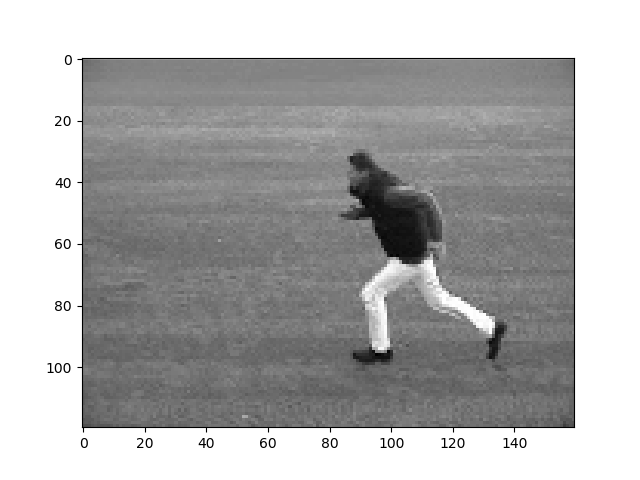
\includegraphics[width=0.3\columnwidth]{frame_gray_1}~
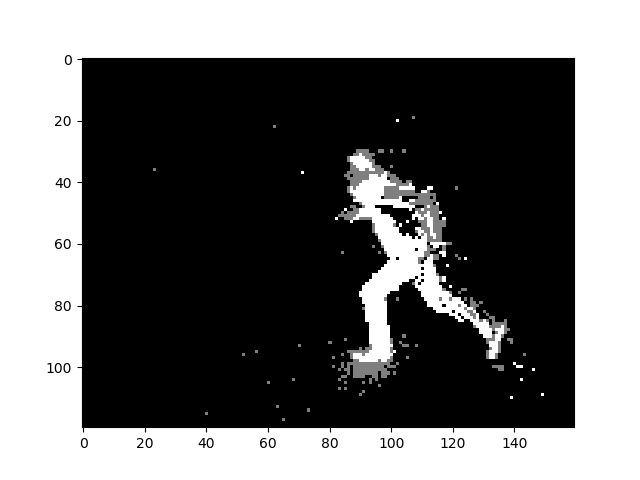
\includegraphics[width=0.3\columnwidth]{fg_mask_1}~
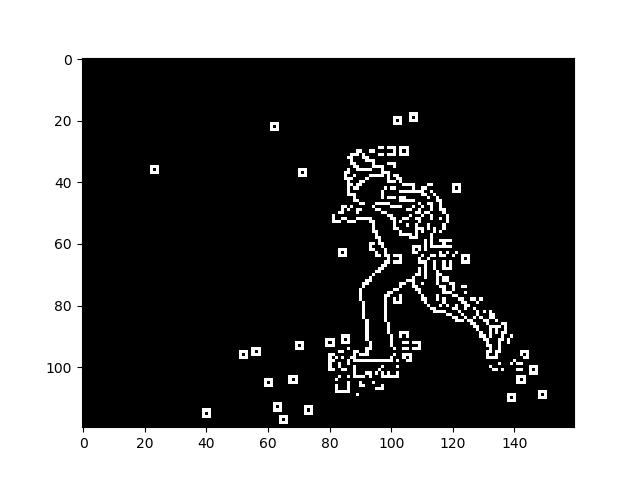
\includegraphics[width=0.3\columnwidth]{edges_1}
\end{subfigure}
\caption{Raw frame, foreground mask, edge image}
\label{fig:images}
\end{figure}

\begin{algorithm}
\caption{Feature Extraction Algorithm}
\begin{algorithmic}[1]
\State For frame $F$ in video:
    \State \indent $G$ $\leftarrow$ grayscaled $F$
    \State \indent Edge image $E$ $\leftarrow$ Canny edge detection on F
    \State \indent Foreground $O$ $\leftarrow$ F minus background
    \State \indent Compute edge features on $O$
    \State \indent Compute centroid features on $O$
    \State \indent Compute optical flow features on $E_{prev}$, $E_{curr}$
\State Use PCA to post-process edge and optical flow features
\State Combine all features into one vector
\end{algorithmic}
\end{algorithm}

\subsection{Model Construction}

As previously described, we train a first-order left-right hidden Markov model for each activity in our dataset. Given a sequence of observed feature vectors, the Baum-Welch algorithm is used to estimate the parameters of the model. A high-level description of the algorithm can be found in Section~\ref{sec:bw-alg}.

\subsection{Video Classification}

We use maximum likelihood estimation in order to classify the activity. In other words, we compute the log probability of a given video's feature vector under each trained HMM, and choose the HMM associated with the highest probability.

On top of MLE, we do two things. First, we ``normalize" the output of each model according to its output statistics over a randomly generated corpus of arbitrary videos. The goal of this step is to make the output distributions of each model resemble each other, so that none have more weight than the others. Second, we borrow a technique from machine learning and ensemble multiple HMMs for each activity. Namely, we train multiple Markov models with varied parameters in a bagging fashion (on different subsamples of the data). As seen in the results section, we find that this provides a slight edge over the vanilla model in most cases.

\section{Experiments}

We train and evaluate our method on videos from the KTH action dataset. The KTH dataset consists of six hundred 160 $\times$ 120 videos, over which six different activities are performed by 25 different people. Conveniently, the videos take place over a homogeneous background; this simplifies the job of background subtraction, which is not the focus of this work.

The six activities included in the dataset are walking, jogging, running, boxing, handwaving, and handclapping. We train a separate HMM for each activity, and judge our algorithm by its multi-class recognition accuracy.

We split the full dataset into a training set of 384 videos and a test set of 216 videos (equating to 64 training videos and 36 test videos per activity).

\section{Results}

Table~\ref{table:results} contains the classification accuracy associated with each of the activities in the KTH dataset. Each percentage denotes the proportion of correctly classified videos for the activity.

\begingroup
\setlength{\tabcolsep}{7pt}
\renewcommand{\arraystretch}{1.3}
\begin{table}[H]
\begin{center}
  \caption{GMM HMMs trained on size-25 edge features and size-25 optical flow features}
  \vspace*{1mm}
  \label{table:results}
  \begin{tabular}{|c|c|c|c|c|c|c|}
    \hline
    Activity & boxing & handclapping & handwaving & jogging & running & walking \\ \hline
    \specialcell{Train \%} & 69\% & 61\% & 58\% & 55\% & 78\% & 70\% \\ \hline
    \specialcell{Test \%} & 61\% & 47\% & 61\% & 53\% & 75\% & 81\% \\ \hline
    \specialcell{Random \%} & 17\% & 17\% & 17\% & 17\% & 17\% & 17\% \\ \hline
  \end{tabular}
\end{center}
\end{table}
\endgroup

Note: since there are six classes, uniform random sampling would yield a classification accuracy of 17\% in expectation. Our method performs quite a bit better than this, showing that it has learned something about each activity.

Table~\ref{table:ensemble} depicts a comparison in classification accuracy between an ensemble-based model and a non-ensemble-based model. The ensemble-based model performs at least as well or better on four of the six activity datasets.

\begingroup
\setlength{\tabcolsep}{7pt}
\renewcommand{\arraystretch}{1.1}
\begin{table}[H]
\begin{center}
  \caption{ensemble of three GMMs trained with different snapshots of the data}
  \vspace*{1mm}
  \label{table:ensemble}
  \begin{tabular}{|c|c|c|c|c|c|c|}
    \hline
    Activity & boxing & handclapping & handwaving & jogging & running & walking \\ \hline
    \specialcell{Test \% \\ (with ensemble)} & 72\% & 52\% & 61\% & 86\% & 52\% & 64\% \\ \hline
    \specialcell{Test \% \\ (without ensemble)} & 61\% & 47\% & 61\% & 53\% & 75\% & 81\% \\ \hline
  \end{tabular}
\end{center}
\end{table}
\endgroup

\section{Discussion}

Our method does relatively well at classifying videos, and significantly outperforms a baseline random model. However, it is far from the state of the art when it comes to human activity recognition. One limitation is that we're using Markov models, which exhibit a memoryless property in that each state depends only on a previous state, whereas newfangled methods utilize more complex models such as LSTMs (which are able to take into account a long-term memory of a sequence, and perhaps understand more about a behavior that way).

If constrained to the domain of Markov, however, the main limitations likely stem from the feature representations we're using. There are many features that could be included that we have not yet tried, e.g. raw flow values in a small window of maximal total flow magnitude, divergence of flow, vorticity of flow, the DFT of distances from the centroid to human contours... the list goes on. Thus far, we have found the feature representation to make the biggest impact on performance.

Furthermore, we have a large number of parameters to tune (see the configuration file in our codebase) and are not quite sure which ones give the best results. We have found that different parameter settings can sway the performance of our model to a large degree, in one instance misclassifying everything and in another classifying everything to a medium ($\sim$40\%) accuracy. Parameters include, e.g., which features to use, dimensionality of feature spaces, number of models in the ensemble, and subsample percentages.

\section{Conclusion}

In this report, we have presented an HMM-based classification approach to human activity recognition. We extend previous approaches with custom-defined feature representations (e.g. PCA ROI edges and histograms of flows), normalization of output distributions, and Markov model ensembles. As alluded to in the previous section, there is much work that could still be done, e.g. re-engineering features and enacting searches over the parameter space for the best values, which we have not yet had the time to do. Nevertheless, on the whole we have found Markov models to give unprecedentedly strong results in the challenging task of activity recognition.

\bibliographystyle{unsrt}
\bibliography{bib}

\end{document}
